\chapter{Injection and Detection Techniques}

\section{Why Injection Matters in Cheat Development}

In the realm of professional game cheating, nearly all serious and commercially available cheats—especially those developed for competitive titles like \textit{Counter-Strike 2}—are built as \textbf{DLLs} that are injected into the game process. This design choice is not incidental; it is fundamental to how modern cheats operate and achieve their functionality.

Injecting a DLL into the game allows the cheat to execute in \textbf{runtime} alongside the game itself. This real-time coexistence grants the cheat direct access to the game's memory, logic, and rendering pipeline. As a result, injected cheats can:

\begin{itemize}
    \item \textbf{Hook internal functions} to intercept or modify game behavior (e.g., aim mechanics, visibility checks).
    \item \textbf{Modify memory values} to influence in-game parameters (e.g., recoil, ammunition, speed).
    \item \textbf{Read game data structures} to extract critical information (e.g., player positions, health, weapons).
    \item \textbf{Render overlays} by drawing directly on top of the game window (e.g., ESP, radar, crosshairs).
    \item \textbf{Automate gameplay} with logic that integrates seamlessly with the game's update loop.
\end{itemize}

This deep integration is only possible through in-process code execution, which is why DLL injection is the industry standard in cheat development. Accordingly, anti-cheat systems like \textbf{Valve Anti-Cheat (VAC)} place significant emphasis on detecting and blocking injection attempts, making injection both the cornerstone of modern cheating and the primary target for detection.

The following sections explore the most relevant injection techniques used in game cheating and the methods employed by anti-cheat systems to detect and prevent them. The objective is to provide a conceptual overview without delving into low-level implementation details.

\section{Overview of Code Injection Techniques}

Code injection refers to the practice of inserting arbitrary executable code into a running process. In the context of cheating, this typically involves loading a custom Dynamic Link Library (DLL) or executing shellcode within the game's memory space to gain persistent and privileged access to game internals.

\subsection*{Traditional Methods}

Early cheats commonly relied on standard Windows functions such as:

\begin{itemize}
    \item \texttt{LoadLibrary}: Loads a DLL into the target process.
    \item \texttt{CreateRemoteThread}: Spawns a new thread in another process to execute injected code.
\end{itemize}

While these approaches are simple and effective in general software development, they are highly detectable. Anti-cheat systems like VAC monitor API usage, track module registrations, and flag suspicious thread creation patterns. As a result, traditional injection methods are now largely ineffective for persistent, undetected cheating.

\subsection*{Manual Mapping}

\textbf{Manual Mapping} has become the preferred method for injecting cheats into modern games. Rather than relying on the Windows loader, this technique manually replicates the steps involved in loading a DLL, entirely within user space.

Manual Mapping is highly effective because:

\begin{itemize}
    \item It bypasses standard API calls like \texttt{LoadLibrary}, avoiding direct detection.
    \item Injected modules do not appear in the target process’s module list (PEB).
    \item Execution can be achieved through stealthy mechanisms such as thread hijacking or shellcode trampolines.
\end{itemize}

Due to its stealth and flexibility, Manual Mapping is considered the most robust and professional method in the current landscape of cheat development.

\section{Detection Techniques in Anti-Cheat Systems}

Anti-cheat engines like VAC continuously scan game processes for indicators of unauthorized code. Their goal is to identify abnormal memory allocations, illegitimate execution paths, or manipulation of trusted system routines.

\subsection*{Thread Local Storage (TLS) Callbacks}

A key detection mechanism involves the use of \textbf{Thread Local Storage (TLS) callbacks}, a feature in the Windows PE (Portable Executable) format that allows developers to specify functions to be executed automatically by the system when threads are created or destroyed, or when the module is loaded or unloaded.

In the context of anti-cheat systems, TLS callbacks are strategically valuable because they are executed \textbf{before the application’s main entry point is reached}, and even \textbf{before asynchronous procedure calls (APCs)} are processed. This early execution allows anti-cheat software to inspect and validate the runtime environment at an extremely privileged stage of process initialization.

\begin{figure}[h!]
    \centering
    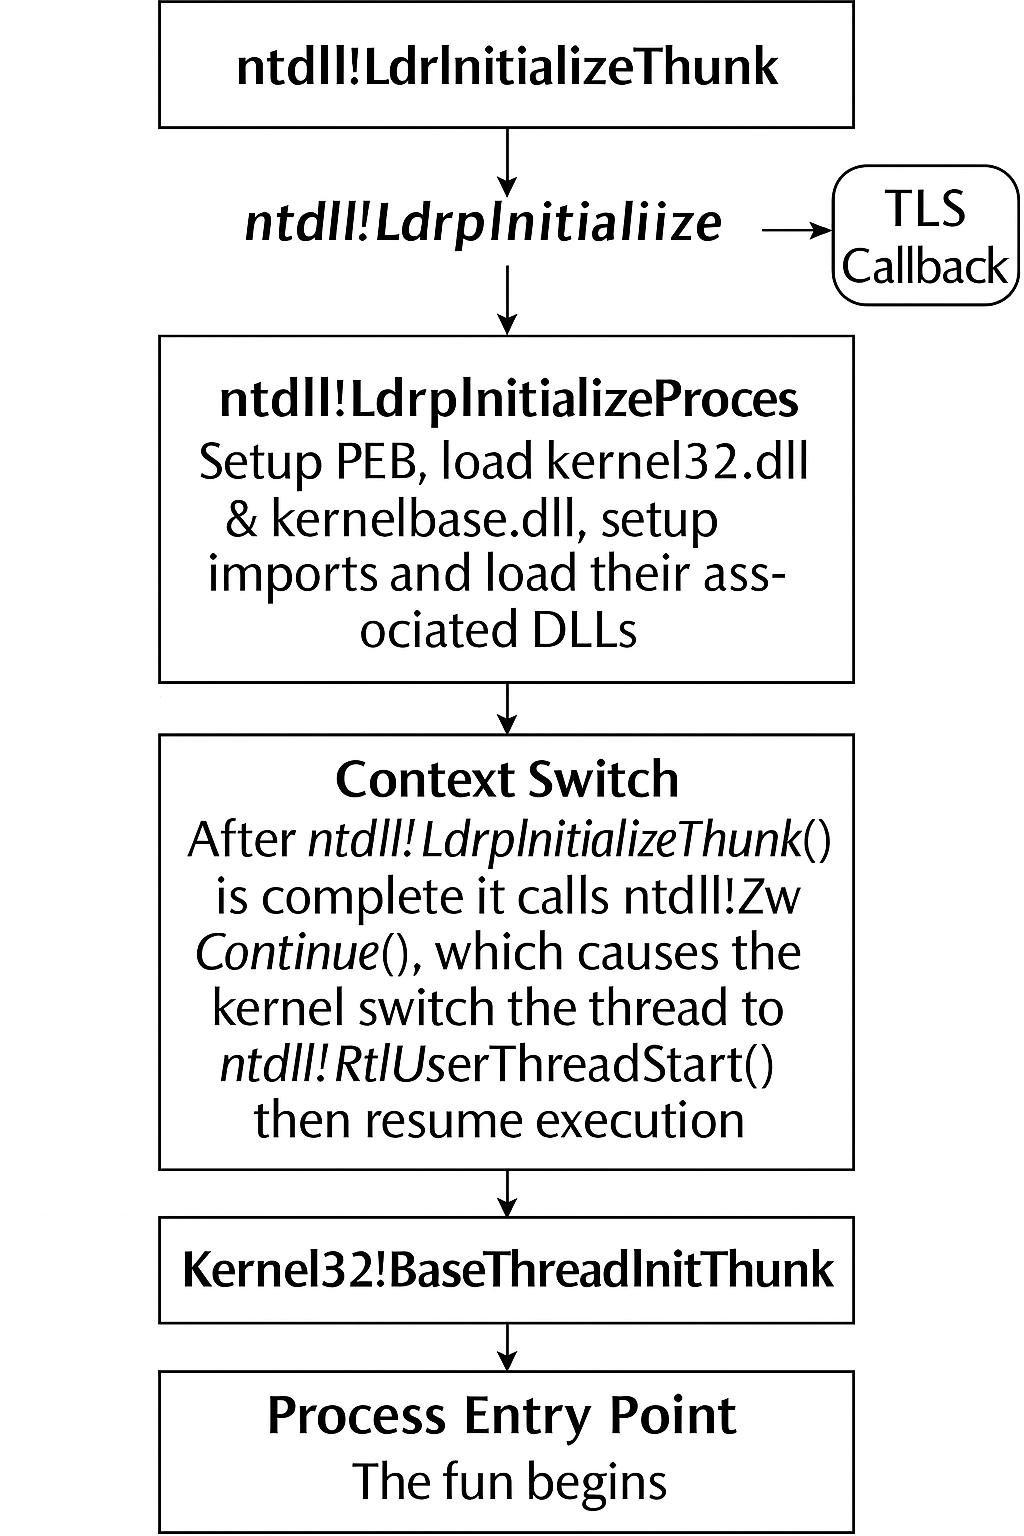
\includegraphics[width=0.45\textwidth]{images/tls_callback.png}
    \caption{Windows thread initialization flow with TLS Callback highlighted.}
    \label{fig:tls-callback-diagram}
\end{figure}

\begin{itemize}
    \item On thread creation, the Windows loader invokes TLS callbacks \textit{within} the routine \texttt{ntdll!LdrpInitializeProcess}, giving anti-cheat DLLs a head start to perform memory integrity checks or verify thread origins.
    \item If an injected DLL includes its own TLS callback, it may be triggered at load time—potentially revealing its presence to the anti-cheat if not properly concealed or removed.
\end{itemize}

Figure~\ref{fig:tls-callback-diagram} illustrates the initialization sequence of a thread in Windows. The TLS callback is highlighted to show its execution point \textbf{before APC dispatch} and \textbf{long before reaching the game’s code}. This makes it a powerful mechanism for early detection of injected modules or tampered execution states.

\vspace{1em}
For cheat developers, understanding the timing of TLS execution is critical. If not disabled or manually stripped from injected DLLs, a TLS callback can inadvertently betray the presence of the cheat before it even begins executing its logic. Consequently, many modern cheats using manual mapping techniques explicitly remove the TLS directory from the PE header to avoid this detection vector.


\subsection*{Start Address Integrity Checks}

Another powerful detection primitive involves analyzing the \textbf{start address} of threads. Threads that begin execution in anonymous memory or outside known game modules are flagged as suspicious. This method is particularly effective against simple shellcode execution or poorly concealed DLL injections.


\subsection*{VMT Hook Detection}

Valve Anti-Cheat (VAC) is capable of detecting manipulations to \textbf{virtual method tables (VMTs)}—a powerful technique commonly used by cheats to hijack the behavior of in-game objects. In object-oriented game engines, many entities expose functionality through virtual methods. By modifying the VMT of such an object, a cheat can effectively redirect calls to its own code, gaining precise control over rendering, physics, and logic routines.

However, VMT hooking leaves detectable traces in memory. Since VMTs are stored in writable memory regions and follow well-defined structural patterns, VAC can perform \textbf{pattern recognition} and \textbf{integrity verification} to identify tampering. This includes checking whether VMT pointers still reference legitimate memory ranges, or if the functions they point to fall outside of expected modules.

\begin{figure}[h!]
    \centering
    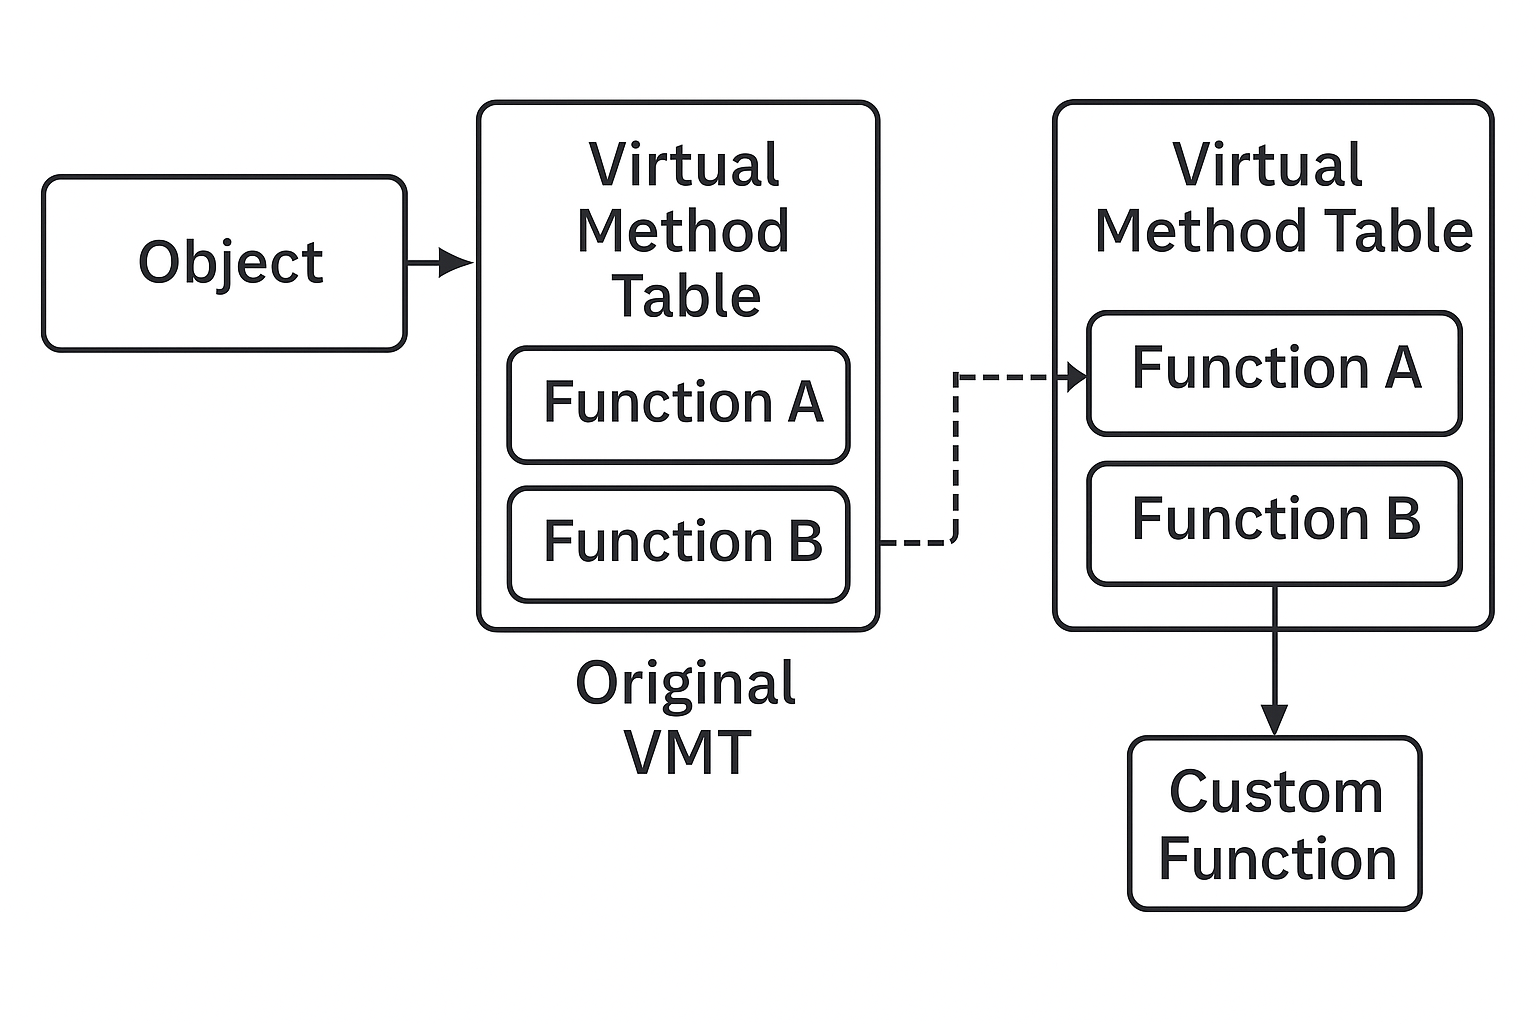
\includegraphics[width=0.65\textwidth]{images/vmthooking.png}
    \caption{Illustration of Virtual Method Table (VMT) Hooking. Function A is redirected to a custom implementation by modifying the object's VMT.}
    \label{fig:vmt-hooking-diagram}
\end{figure}

To evade detection, some cheats attempt to clone the original VMT, apply hooks to the clone, and then swap the object’s VMT pointer. Others periodically restore and reapply the hook depending on the scan timing. In more recent developments, some developers have abandoned VMT hooking altogether in favor of inline detours or Return-Oriented Programming (ROP) chains, which are harder to attribute to specific objects.


\section{Evasion Techniques Used by Cheats}

To remain undetected, cheat developers employ advanced evasion strategies. These techniques are specifically designed to circumvent TLS callbacks, start address validation, and memory integrity checks.

\subsection*{Suppressing TLS Callbacks}

One method to bypass TLS-based detection is to remove or disable the TLS callback table in the injected DLL. This can be achieved by:

\begin{itemize}
    \item Manually modifying the PE header to erase TLS structures.
    \item Avoiding the use of new threads, thus preventing callback invocation.
\end{itemize}

\subsection*{Thread Hijacking and Return Address Spoofing}

\textbf{Thread hijacking} avoids the creation of new threads by taking control of an existing game thread. The cheat suspends a legitimate thread, modifies its instruction pointer, and redirects it to execute the injected payload.

To further mask execution, cheats employ \textbf{return address spoofing}, which fakes the origin of a function call. By placing a plausible return address on the stack, the cheat deceives anti-cheats into believing that execution flow originated from a legitimate module.



\subsection*{Start Address Redirection via ROP Gadgets}

A sophisticated method employed by cheat developers to circumvent return address validation is through the use of \textbf{ROP (Return-Oriented Programming) gadgets}. These are short instruction sequences that already reside in memory regions of trusted modules—such as the game binary or linked system libraries—and typically end in control transfer instructions like \texttt{ret}, \texttt{jmp reg}, or similar.

Instead of making a direct call to untrusted or injected code (which would be easily detected through stack tracing), the cheat sets up a \emph{call stub} that emulates a legitimate function call. This stub pushes a spoofed return address onto the stack—pointing to a trusted gadget—and then jumps to the target function. The result is an execution flow that appears legitimate during runtime analysis, effectively evading static return address checks commonly used by anti-cheat solutions like Valve Anti-Cheat (VAC).

\paragraph{Stack Alignment and Shadow Space.} To maintain runtime stability and comply with Windows x64 calling conventions, the stub must properly align the stack and allocate shadow space (32 bytes) for callees. A minimal x64 stub might resemble the following:
\begin{lstlisting}[style=asmstyle]
sub rsp, 0x28               ; align stack and reserve shadow space
mov rax, 0xFFAAFFAAFFAAFFAA ; spoofed return address (ROP gadget)
push rax
mov rax, 0xFFAAFFAAFFAAFFAA ; actual target function
jmp rax
\end{lstlisting}

\paragraph{Gadget Selection.} 

A ROP gadget is typically a short instruction sequence ending in a control-transfer instruction, like \texttt{ret} or \texttt{jmp reg}. These gadgets already exist within the code section of loaded modules (usually the \texttt{.text} section), making them ideal for stealth execution. Rather than injecting new code, the attacker reuses these sequences to craft a control flow that appears legitimate.

Gadget discovery is usually performed via \emph{pattern scanning}, where the cheat scans memory regions of trusted modules (e.g., the game binary or system DLLs) to identify usable byte sequences. This is done by matching instruction patterns known to safely clean up the stack or transfer execution.

The goal is to find gadgets that:
\begin{itemize}
    \item Correct the stack pointer (\texttt{rsp} or \texttt{esp}) to undo shadow space or argument pushes.
    \item Preserve or restore registers, avoiding clobbering values needed by the callee.
    \item Cleanly return to the next address on the stack (spoofed or legitimate).
\end{itemize}

Below are common x64 gadget patterns that fulfill these requirements:
\begin{lstlisting}[style=asmstyle]
add rsp, 0x28
ret
\end{lstlisting}
This gadget restores the stack pointer by skipping over the shadow space (32 bytes), then returns. It's ideal for restoring alignment after a spoofed call.

\begin{lstlisting}[style=asmstyle]
pop rcx
add rsp, 0x20
ret
\end{lstlisting}
This variant additionally pops a register (which might be part of a cleanup routine), followed by stack adjustment and a return.

\begin{lstlisting}[style=asmstyle]
add rsp, 0x20
pop rax
jmp rax
\end{lstlisting}
Instead of returning, this gadget transfers control directly to an address stored in \texttt{rax}. It's often used as a trampoline when returning via \texttt{ret} is too risky or when control needs to flow to shellcode.

These gadgets are typically located by scanning for their machine code representations (byte signatures) in memory. Once identified, they are hardcoded or dynamically resolved at runtime, depending on the injection strategy.


\paragraph{x86 Considerations.} On x86 systems, spoofing becomes more nuanced due to the variety of calling conventions in use \texttt{\_cdecl}, \texttt{\_thiscall}, and \texttt{\_fastcall}, among others. Each convention has its own argument-passing semantics and stack cleanup behavior. Below is an example of a stub for a \texttt{\_thiscall} function:
\begin{lstlisting}[style=asmstyle]
sub esp, 0x0C
mov eax, 0xFFAAFFAA        ; spoofed return address
mov [esp], eax
mov eax, [esp+0x10]
mov [esp+4], eax
mov eax, [esp+0x14]
mov [esp+8], eax
mov eax, 0xFFAAFFAA        ; actual target function
jmp eax
\end{lstlisting}

Here, the return address is spoofed and the arguments are manually arranged on the stack to match the callee's expected layout.

\paragraph{Detection Vectors.} Although this technique can bypass static stack validation, it is not impervious to detection. Anti-cheat engines can perform \textbf{stack walking}—analyzing the call stack at runtime—to identify anomalies such as unexpected return addresses or invalid module references. To counteract this, some cheats implement post-call cleanup via chained gadgets or trampolines that restore a believable call chain before returning.

\paragraph{Practical Implementations.} Open-source projects like \texttt{x86RetSpoof} by danielkrupinski encapsulate these techniques in reusable tooling for x86-based games. However, bespoke implementations remain common in private cheat circles, especially in paid cheats (\textit{P2C}) for titles like CS:GO and CS2.







\section{Extended VAC Capabilities and Developer Countermeasures}

Beyond memory inspection and thread analysis, VAC includes a broader set of capabilities that significantly increase its detection surface.

\subsection*{Observed Detection Capabilities}

Community research and reverse engineering have revealed that VAC likely performs:

\begin{itemize}
    \item \textbf{File System Scanning}: Searches for known cheat artifacts and patterns.
    \item \textbf{Process and Memory Scanning}: Inspects all running processes for injection, shellcode, and suspicious modules.
    \item \textbf{Registry Inspection}: Identifies unusual startup entries or configuration keys.
    \item \textbf{Handle Enumeration}: Flags abnormal access to game-related objects.
    \item \textbf{Hook and Signature Scanning}: Detects common hook patterns and byte signatures from known cheat loaders.
\end{itemize}

These mechanisms work in concert with behavioral monitoring and cloud-based analysis, making VAC highly resilient to static evasion alone.

\subsection*{Common Countermeasures Used by Cheat Developers}

In response, professional cheat developers implement an array of countermeasures designed to reduce their attack surface and mislead detection heuristics:

\begin{itemize}
    \item \textbf{String Encryption}: Prevents signature-based scanning of identifiable strings.
    \item \textbf{Window and Module Name Randomization}: Avoids static blacklisting and manual heuristics.
    \item \textbf{Polymorphic Code}: Constantly mutates the cheat’s binary structure to evade pattern recognition.
    \item \textbf{Fileless Execution}: Prevents disk-based detection by streaming the cheat entirely into memory.
    \item \textbf{Memory Cleansing}: Removes metadata and headers after injection to eliminate identifiable traces.
    \item \textbf{Registry Hygiene}: Ensures no persistent keys or logs remain after execution.
    \item \textbf{Scan Spoofing}: Hooks or replaces VAC scanning routines with fake responses to conceal activity.
\end{itemize}

These techniques are essential for achieving long-term undetectability in highly monitored environments such as Valve’s matchmaking infrastructure.


DLL injection remains the foundation of modern cheat development in competitive games. Techniques such as Manual Mapping offer powerful stealth capabilities, enabling deep integration with the game runtime. However, anti-cheat systems like VAC employ increasingly sophisticated detection methods, including TLS callbacks, memory integrity scanning, VMT hook detection, and behavioral analysis.
